\documentclass[fontsize=12pt,
% headinclude,
 twoside=false, parskip=half+, numbers=noenddot, plainheadsepline, toc=listof
 %, toc=bibliography
 ]{scrreprt}
% PDF-Kompression
\pdfminorversion=5
\pdfobjcompresslevel=1
% Allgemeines
\usepackage[automark]{scrpage2} % Kopf- und Fußzeilen
\usepackage{amsmath,marvosym} % Mathesachen
\usepackage[T1]{fontenc} % Ligaturen, richtige Umlaute im PDF
\usepackage[utf8]{inputenc}% UTF8-Kodierung für Umlaute usw

\usepackage{geometry}
\geometry{a4paper,left=50mm,right=30mm, top=1cm, bottom=2cm}
% Schriften
\usepackage{mathpazo} % Palatino für Mathemodus
%\usepackage{mathpazo,tgpagella} % auch sehr schöne Schriften
\usepackage{setspace} % Zeilenabstand
\onehalfspacing % 1,5 Zeilen
% Schriften-Größen
\setkomafont{chapter}{\Large\rmfamily} % Überschrift der Ebene
\setkomafont{section}{\large\rmfamily}
\setkomafont{subsection}{\rmfamily}
\setkomafont{subsubsection}{\rmfamily}
\setkomafont{chapterentry}{\large\rmfamily} % Überschrift der Ebene in Inhaltsverzeichnis
\setkomafont{descriptionlabel}{\bfseries\rmfamily} % für description Umgebungen
\setkomafont{captionlabel}{\small\bfseries}
\setkomafont{caption}{\small}
% Sprache: Deutsch
\usepackage[ngerman]{babel} % Silbentrennung
% PDF
\usepackage[ngerman]{hyperref}
\usepackage[final]{microtype} % mikrotypographische Optimierungen
\usepackage{url}
\usepackage{pdflscape} % einzelne Seiten drehen können
% Tabellen
\usepackage{multirow} % Tabellen-Zellen über mehrere Zeilen
\usepackage{multicol} % mehre Spalten auf eine Seite
\usepackage{tabularx} % Für Tabellen mit vorgegeben Größen
\usepackage{longtable} % Tabellen über mehrere Seiten
\usepackage{array}
%  Bibliographie
%\usepackage{bibgerm} % Umlaute in BibTeX
% Tabellen
\usepackage{float}
\usepackage{wrapfig}
% Bilder
\usepackage{graphicx} % Bilder
\usepackage{color} % Farben
\usepackage{colortbl}%Hintergrundfarben für Tabellen	
% Define user colors using the RGB model
\definecolor{dunkelgrau}{rgb}{0.8,0.8,0.8}
\definecolor{hellgrau}{rgb}{0.95,0.95,0.95}
\definecolor{red}{rgb}{1.0,0.5,0.5}
\graphicspath{{images/}}
\DeclareGraphicsExtensions{.pdf,.png,.jpg} % bevorzuge pdf-Dateien
\usepackage{subfigure} % mehrere Abbildungen nebeneinander/übereinander
\newcommand{\subfigureautorefname}{\figurename} % um \autoref auch für subfigures benutzen
\usepackage[all]{hypcap} % Beim Klicken auf Links zum Bild und nicht zu Caption gehen
% Bildunterschrift
\setcapindent{0em} % kein Einrücken der Caption von Figures und Tabellen
\setcapwidth[c]{0.9\textwidth}
\setlength{\abovecaptionskip}{0.2cm} % Abstand der zwischen Bild- und Bildunterschrift
% Quellcode
\usepackage{listings} % für Formatierung in Quelltexten
\definecolor{grau}{gray}{0.25}
\definecolor{lightgray}{rgb}{.9,.9,.9}
\definecolor{darkgray}{rgb}{.4,.4,.4}
\definecolor{purple}{rgb}{0.65, 0.12, 0.82}

\lstdefinelanguage{JavaScript}{
  keywords={typeof, new, true, false, catch, function, return, null, catch, switch, var, if, in, while, do, else, case, break},
  keywordstyle=\color{blue}\bfseries,
  ndkeywords={class, export, boolean, throw, implements, import, this},
  ndkeywordstyle=\color{darkgray}\bfseries,
  identifierstyle=\color{black},
  sensitive=false,
  comment=[l]{//},
  morecomment=[s]{/*}{*/},
  commentstyle=\color{purple}\ttfamily,
  stringstyle=\color{red}\ttfamily,
  morestring=[b]',
  morestring=[b]"
}
\lstset{
   language=JavaScript,
   backgroundcolor=\color{lightgray},
   extendedchars=true,
   basicstyle=\scriptsize\ttfamily,
   showstringspaces=false,
   showspaces=false,
   %numbers=right,
   numberstyle=\scriptsize\ttfamily,
   numbersep=9pt,
   tabsize=2,
   breaklines=true,
   showtabs=false,
   captionpos=b
}
%\lstset{
%	extendedchars=true,
%	%basicstyle=\small\ttfamily,
%	language=java,
%	basicstyle=\footnotesize\ttfamily,
%	tabsize=2,
%	keywordstyle=\textbf,
%	commentstyle=\color{grau},
%	stringstyle=\textit,
%	numbers=left,
%	numberstyle=\small,
%	% für schönen Zeilenumbruch
%	breakautoindent  = true,
%	breakindent      = 2em,
%	breaklines       = true,
%	postbreak        = ,
%	prebreak         = \raisebox{-.8ex}[0ex][0ex]{\Righttorque},
%}
% linksbündige Fußboten
\deffootnote{1.5em}{1em}{\makebox[1.5em][l]{\thefootnotemark}}

%\typearea{14} % typearea am Schluss berechnen lassen, damit die Einstellungen oben berücksichtigt werden
% für autoref von Gleichungen in itemize-Umgebungen
\makeatletter
\newcommand{\saved@equation}{}
\let\saved@equation\equation
\def\equation{\@hyper@itemfalse\saved@equation}
\makeatother 


 % Importiere die Einstellungen aus der Präambel
% hier beginnt der eigentliche Inhalt
\begin{document}
\pagenumbering{Roman} % große Römische Seitenummerierung
\pagestyle{empty}

% Titelseite
\clearscrheadings\clearscrplain

\begin{center}
\begin{Huge}
Institut für Mathematik und Informatik\\
\vspace{3mm}
\end{Huge}{\Large Fernuniversiät Hagen}\\

\vspace{20mm}
\begin{Large}
Vergleichende Implementierung und Evaluierung einer ereignisgesteuerten, nicht
blockierenden I/O Lösung für eine datenintensive Real-Time Webanwendung in Javascript
und Dart\\
\end{Large}
\vspace{8mm}
Bachelorarbeit\\
\vspace{0.4cm}
\vspace{2 cm}
Barbara Drüke \\
Matrikel-Nummer 7397860\\
\vspace{5cm}
\begin{tabular}{ll}
{\bf Betreuer} & Dr. Jörg Brunsmann\\
{\bf Erstprüfer}&Prof. Hemmje\\
{\bf Zweitprüfer}&Dr. Jörg Brunsmann\\
\end{tabular}

\end{center}
\clearpage


\pagestyle{useheadings} % normale Kopf- und Fußzeilen für den Rest

\tableofcontents
\listoffigures
\listoftables





% richtiger Inhalt
%---------------------------------------------------------------------------------------------------------------------------------------------
\chapter{Einleitung}
\pagenumbering{arabic} % ab jetzt die normale arabische Nummerierung

Die Vesseltracker.com GmbH ist ein Schiffsmonitoring und -reporting-Dienstleister. Der kostenpflichtige Dienst stellt den Kunden umfangreiche Informationen zu Schiffen weltweit zur Verfügung. Dabei handelt es sich einerseits um Schiffs-Stammdaten und andererseits um Schiffs-Postionsdaten. Die Positionsdaten sind AIS (Automatic Identification System) -Daten, wie sie von allen Schiffen über Funk regelmäßig zu senden sind.

\begin{wrapfigure}{r}{0.6\textwidth}
  \begin{center}
    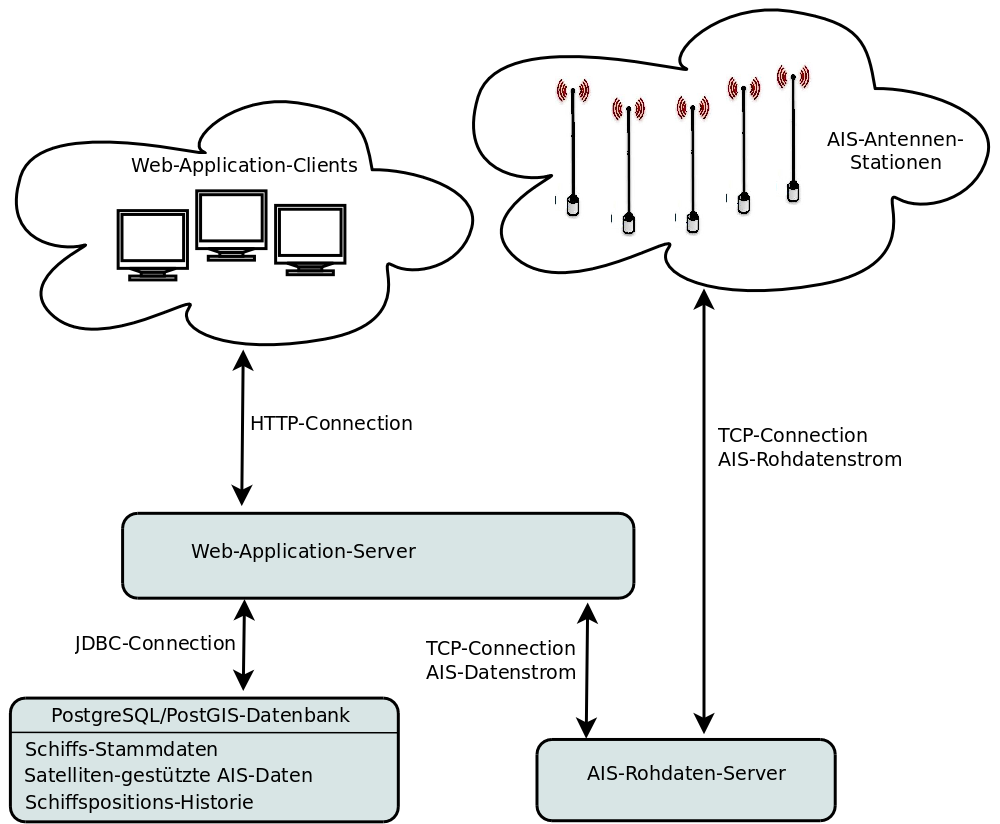
\includegraphics[width=0.58\textwidth]{images/Exposee_graphik_Webapp}
  \end{center}
  \caption{Vesseltracker\_Webapplikation}
\end{wrapfigure}

Vesseltracker.com unterhält ein Netzwerk von ca. 800 terrestrischen AIS-Antennen, mit denen küstennahe AIS-Meldungen empfangen und via Internet an einen zentralen Rohdatenserver geschickt werden. Der Rohdatenserver verarbeitet die Meldungen und gibt sie umgewandelt und gefiltert an die Anwendungen des Unternehmens weiter.
Zusätzlich erhält das Unternehmen AIS-Daten via Satellit über einen Kooperationspartner. Damit werden die küstenfernen Meeresgebiete und Gegenden, in denen Vesseltracker.com keine AIS-Antenne betreibt, abgedeckt.
Die Kernanwendung des Unternehmens ist eine Webanwendung, die die terrestrischen AIS-Daten in einer Geodatenbank speichert und sie mit den Schiffs-Stammdaten und Satelliten-AIS-Daten in Beziehung setzt.

Für eine geographische Visualisierung der Schiffspositionen existiert das sogenannte 'Cockpit', wo die Schiffe als Icons auf Openstreetmap-Karten dargestellt werden. Diese Karte zeigt jeweils alle Schiffe an, die sich in dem frei wählbaren Kartenausschnitt zu der Zeit befinden. Aktualisiert werden die Positionsinformationen jeweils bei Änderung des betrachteten Bereichs oder einmal pro Minute. Detailinformationen erhält der Nutzer durch ein Click-Popup über das Icon des Schiffes. Darüber kann er sich auch die gefahrene Route der letzten 24 h anzeigen lassen.


\begin{figure}[H]
  \centering
  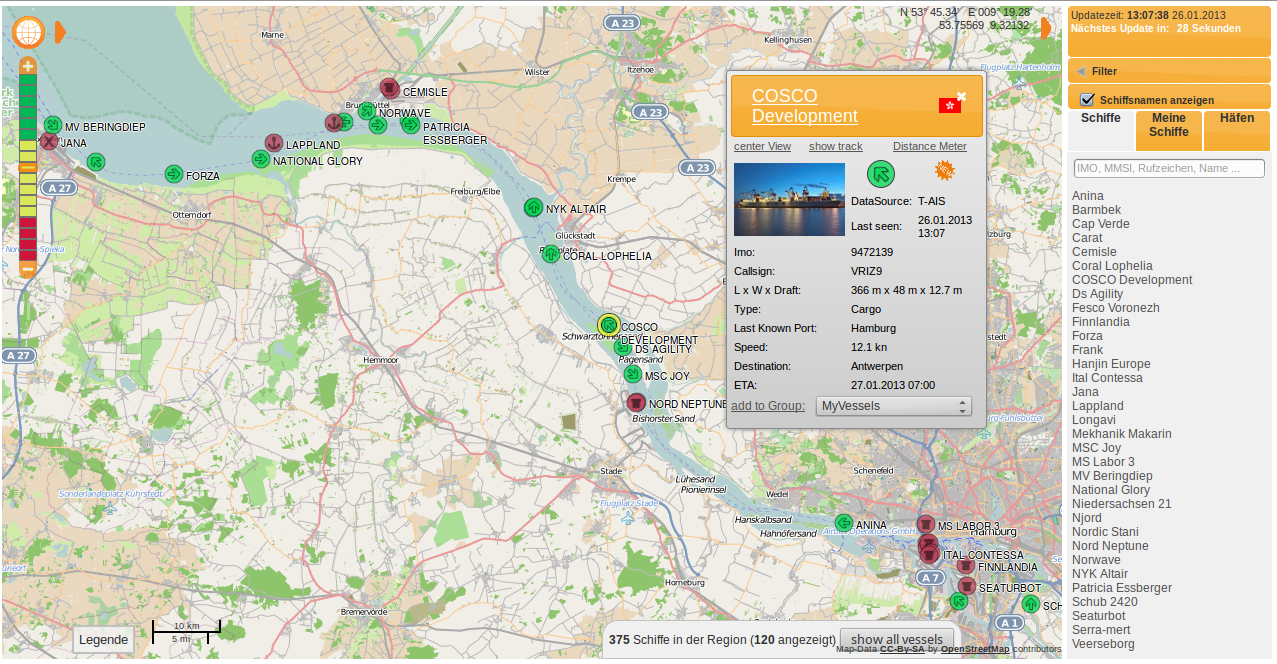
\includegraphics[width=6in]{images/Cockpit_Elbe}
  \caption[Cockpit\_Elbe]{Cockpit\_Elbe}
\end{figure}

\section{Motivation für diese Arbeit}\label{s.Motivation für diese Arbeit}

Aus mehreren Gründen erscheint es angebracht, die geographischen Schiffspositionen nicht nur über die Cockpit-Anwendung anzubieten, sondern alternativ als real-time-Darstellung. 
\begin{itemize}

\item Aufgrund der herausragenden Qualität des vesseltracker.com Antennen-Netzwerks sind die verfügbaren AIS-Daten aktuell, aktualisieren sich kontinuierlich und erreichen eine hohe weltweite Abdeckung. Damit ist es möglich, die Schiffsverkehrslage beliebiger Häfen, Wasserstraßen, Küstengebiete weltweit und sekundengenau zu präsentieren. 

\item Ein Phänomen in der menschlichen Wahrnehmung lässt die geplante Anwendung sehr viel zweckmäßiger erscheinen als die bisherige Cockpit-Anwendung. Aufgrund der sogenannten Veränderungsblindheit oder “Change Blindness” werden Veränderungen an einem Objekt (in diesem Fall die Position eines Schiffs-Icons auf der Karte) in der Wahrnehmung überdeckt, wenn im selben Augenblick Veränderungen an der Gesamtsicht vonstatten gehen. Im Cockpit werden nach dem Laden neuer Positionsdaten alle Schiffsicons neu gerendert und unter Umständen Namens-Fähnchen gelöscht oder hinzugefügt, was zu einem kurzen “Flackern” führt. Dadurch ist es dem Betrachter nahezu unmöglich, die Positionsänderung eines Schiffes auf der Karte nachzuvollziehen.
  
\item Real-time-Anwendungen gewinnen zunehmend an Bedeutung. Ihre Verbreitung wird durch den Fortschritt der verfügbaren Webtechnologien auf breiter Basis unterstützt. Mitbewerber auf dem Markt für AIS-Daten (z.B. Fleetmon.com) bieten bereits Echtzeit-Darstellungen ihrer AIS-Daten an. Um in diesem Geschäftsfeld weiterhin eine Spitzenposition innezuhaben, ist eine Realtime zwingend erforderlich, in einem nächsten Schritt sicher auch als Anwendung für Mobile Devices.
\end{itemize}


\section{Aufbau der Arbeit}\label{s.Aufbau der Arbeit}
Im Kapitel 2 werden mögliche Anwendungs-Szenarien genauer beleuchtet und die funktionalen und nicht funktionalen Anforderungen an die geplante Anwendung herausgestellt. Anschließend wird die Systemarchitektur der geplanten Anwendung grob entworfen.
Kapitel 3.1 gibt eine kurze Einführung in die Websocket-Technologie, Kapitel 3.2 stellt die Programmiersprache Google Dart vor.
In Kapitel werden zunächst die Gründe für die getroffene Auswahl an Implementierungen dargelegt und anschließend die Vorgehensweise bei der Implementierung erläutert. Die Implementierungen werden auszugsweise vorgestellt.
Die ausgearbeiteten Implementierungen werden dann in Kapitel 5 getestet und nach verschiedenen Aspekten verglichen.
Kapitel 6 fasst die Ergebnisse zusammen.

%---------------------------------------------------------------------------------------------------------------------------------------------
\chapter{Realtime-Schiffsverfolgung per AIS-Daten-Strom}\label{c.Realtime-Schiffsverfolgung per AIS-Daten-Strom}

\section{ Anwendungsfälle}\label{s.Anwendungsfälle}

Hafendienstleister wie Schlepper, Lotsen oder Festmacher verschaffen sich über einen Monitor einen Überblick über die Arbeitsvorgänge in ihrem jeweiligen Heimathafen, z.B. welche Schlepper welches Schiff schleppen, wo Lotsen an oder von Bord gehen, von welchen Tankern Schiffe betankt werden. Sie kontrollieren die eigenen Aufträge oder auch die der Mitbewerber.
Die Anwendung läuft hierbei eher statisch, das heißt Zoomstufe und Kartenausschnitt ändern sich nur selten. Es ist also notwendig, dass die Anwendung unabhängig von Aktionen des Nutzers sich laufend oder regelmäßig aktualisiert.

Reedereien beobachten das Einlaufen, Anlegen, Festmachen, Ablegen und Auslaufen ihrer Schiffe in entfernten Häfen, wo es keine Unternehmensniederlassung gibt. Zum Beispiel kontrollieren sie, wann, an welchen Liegeplätzen ein Schiff wie lange festmacht.
Dazu ist es zum einen notwendig, jederzeit auf eine geringe Zoomstufe heraus- und auf einen anderen Hafen wieder hineinzoomen zu können. Zum anderen soll die Anwendung Schnittstellen bieten, damit zusätzliche Informationen aus dem vesseltracker.com Datenpool (in diesem Fall Liegeplatzinformationen) von der Anwendung abgerufen werden können.

Weitere Anwendungsfälle sind Nutzer aus der Passagierschifffahrt, Schiffsfotografen oder Sicherheitsorgane (z.B. die Wasserschutzpolizei), bei denen die Beobachtung / Überwachung bestimmter Wasserverkehrswege oder Häfen von besonderem Interesse ist.

Die vesseltracker.com GmbH nutzt die Realime-Anwendung, um die vom Unternehmen angebotenen Daten zu präsentieren und zu bewerben. Dabei ist es wichtig, dass die Anwendung gesendete AIS-Signale im Schnitt in weniger als einer Sekunde auf dem Monitor als Position oder Positionsänderung darstellen kann und dass die Schiffsbewegungen fließend ohne das in der Einleitung beschriebene “Flackern” dargestellt werden. Damit kann vesseltracker.com die höhere Genauigkeit und Aktualität der eigenen Daten gegenüber denen anderer Anbieter herausstellen.

Die Anwendungsfälle verdeutlichen noch einmal, dass der zusätzliche Nutzen der Realtimeanwendung gegenüber der Cockpitanwendung nicht ausschließlich im Informationsgehalt liegt. Die Daten im Cockpit sind ja ebenfalls im Minutenbereich aktuell. Der Vorteil liegt vielmehr in der Lebendigkeit der Darstellung. Bewegte Darstellungen binden stärker und für einen längeren Zeitraum die Aufmerksamkeit des Betrachters.

\section{Beschreibung der Anforderungen}\label{s.Beschreibung der Anforderungen}

Die funktionalen Anforderungen sind:
\begin{itemize}

\item als Datenquelle sollen ausschließlich die vom Rohdatenserver als JSON-Datenstrom zur Verfügung gestellten AIS-Informationen dienen
\item Schiffe sollen an ihrer aktuellen (realtime) Position auf einer Karte im Browser dargestellt werden
\item Positionsänderungen einzelner Schiffe sollen ad hoc sichtbar gemacht werden
\item die Schiffsbewegungen auf der Karten sollen nicht sprunghaft, sondern fließend erscheinen (Animation der Schiffsbewegungen in dem Zeitraum zwischen zwei Positionsmeldungen)
\item die Karte soll in 16 Zoomstufen die Maßstäbe von 1:2000 bis 1: 200 Mio abdecken
\item Schiffe sollen auf der Karte als Icons dargestellt werden, die den Navigationsstatus und gegebenenfalls den Kurs wiederspiegeln
\item bei hoher Auflösung und ausreichend statischen AIS-Informationen soll ein Schiff als Polygon in die Karte eingezeichnet werden.
\item bei geringer Auflösung ist ein Überblick über die Verteilung der empfangenen Schiffe zu vermitteln
\item Detail-Informationen zu jedem Schiff sollen als Popups über das Icon abrufbar sein
\end{itemize}

Nicht funktionale Anforderungen sind:
\begin{itemize}
\item die von den Antennen empfangenen AIS-Daten sind mit minimaler Verzögerung (< 500 msec) auf der Karte darzustellen
\item die Anwendung sollte ca. 300 Verbindungen gleichzeitig erlauben und skalierbar sein
\item als Clients der Anwendung sollten die gängigsten Browser unterstützt werden (IE, Chrome, Firefox, Safari, Opera) 
\item die Implementierungen werden auf Github als privates repository gehalten
\item als Kartenmaterial sind die von vesseltracker gehosteten OpenstreetMap-Karten zu verwenden
\item verwendete Software-Module sollten frei zugänglich sein (open source) 
\item ein Prototyp der Anwendung soll schnell zur Verfügung stehen. Dieser Prototyp soll Mitarbeitern und Partnern ermöglichen, ihre Anforderungen genauer zu spezifizieren oder sogar neue Anforderungen zu formulieren. 
\end{itemize}

\section{Grobentwurf der Anwendung}\label{s.Grobentwurf der Anwendung}

\begin{wrapfigure}{r}{0.6\textwidth}
  \begin{center}
    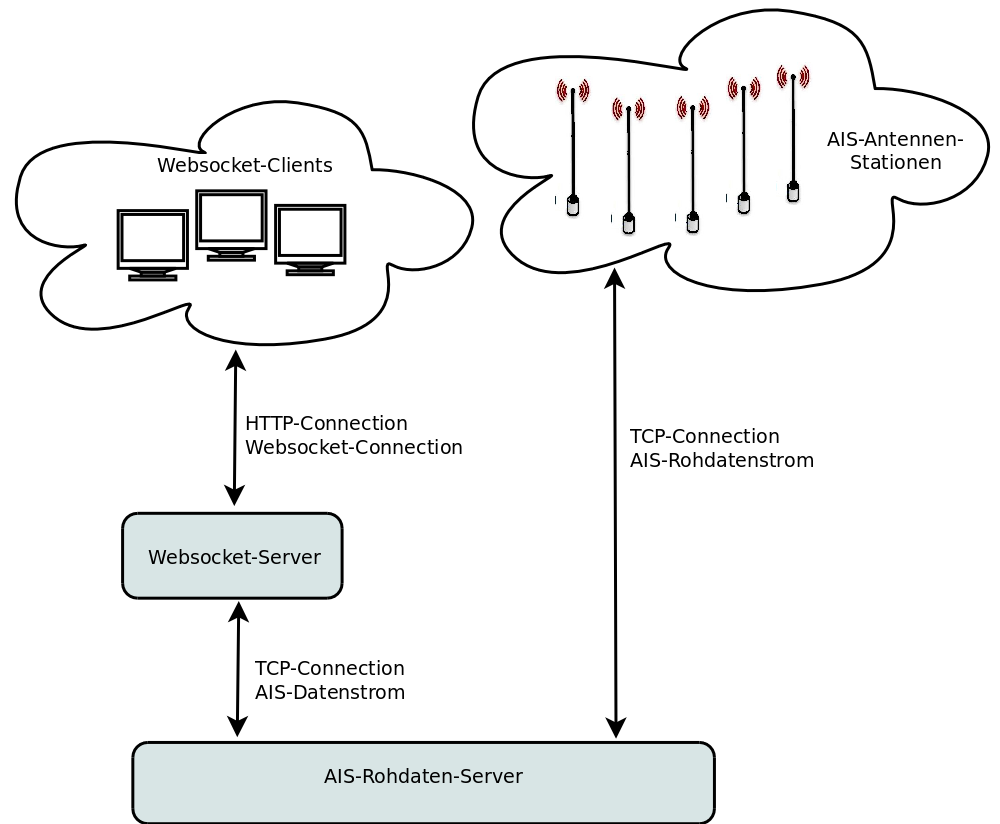
\includegraphics[width=0.58\textwidth]{images/Exposee_graphik_Realtimeapp}
  \end{center}
  \caption{Architektur-Entwurf der Realtime Webapplikation}
\end{wrapfigure}
Die eingehende Schnittstelle der zu erstellenden Anwendung ist die Verbindung zum Rohdatenserver, die als TCP-Verbindung ausgeführt ist und einen JSON-Datenstrom liefert.
Die ausgehende Schnittstelle ist der HTTP-Client (Browser).
Zu erstellen ist also eine Client-Server-Anwendung, in der der Server zweifaches zu leisten hat, nämlich 
\begin{enumerate}
 \item eine tcp-socket-Verbindung zum Rohdatenserver zu unterhalten und
  \item eine bidirektionale Verbindung zum HTTP-Client zu halten, in der der Client jederzeit Änderungen des betrachteten Kartenausschnittes an den Server senden und der Server jederzeit den Client über relevante, aus dem JSON-Datenstrom ausgelesene, Schiffsbewegungen im betrachteten Kartenausschnitt informieren kann.
\end{enumerate}


%---------------------------------------------------------------------------------------------------------------------------------------------
\chapter{Grundlagen}\label{s.Grundlagen}
\section{Automatisches Informationssystem}\label{s.Automatisches Informationssystem (AIS)}
Das Automatic Identification System (AIS) ist ein UKW-Funksystem im Schiffsverkehr, das seit 2004 für alle Berufsschiffe über 300 BRZ in internationaler Fahrt und seit 2008 auch für solche über 500 BRZ in nationaler Fahrt verpflichtend eingeführt worden ist. Es soll dabei helfen, Kollisionen zwischen Schiffen zu verhüten und die landseitige Überwachung und Lenkung des Schiffsverkehrs zu erleichtern. Außerdem verbessert AIS die Planung an Bord, weil nicht nur Position, Kurs und Geschwindigkeit der umgebenden Schiffe übertragen werden, sondern auch Schiffsdaten (Schiffsname, MMSI-Nummer, Funkrufzeichen, etc.). AIS ist mit UKW-Signalen unabhängig von optischer Sicht und Radarwellenausbreitung.\\
Für die Nutzung von AIS ist ein aktives, technisch funktionsfähiges Gerät an Bord Voraussetzung, das sowohl Daten empfängt als auch Daten sendet. Für Schiffe der Berufsschifffahrt sind Klasse-A-Transceiver an Bord vorgesehen, für nicht ausrüstungspflichtige Schiffe genügen Klasse-B-Transceiver, die mit niedriger VHF-Signalstärke und weniger häufig senden.  \\
Die dynamischen Schiffsdaten (LAT, LON, COG, SOG, UTC) erhält der AIS-Transceiver vom integrierten GPS-Empfänger, bei Klasse A auch von der Navigationsanlage des Schiffes. Die Kursrichtung (Heading =  HDG) kann über eine NMEA-183-Schnittstelle vom Kompass eingespeist werden.

Die AIS-Einheit sendet schiffsspezifische Daten, die von jedem AIS-Empfangsgerät in Reichweite empfangen und ausgewertet werden können:
\subsubsection{Statische Schiffsdaten} \label{Statische Schiffsdaten}
\begin{itemize}
\item IMO-Nummer
\item Schiffsname
\item Rufzeichen
\item MMSI-Nummer
\item Schiffstyp (Frachter, Tanker, Schlepper, Passagierschiff, SAR, Sportboot u. a.)
\item Abmessungen des Schiffes (Abstand der GPS-Antenne von Bug, Heck, Backbord- und Steuerbordseite)
\end{itemize}

\subsubsection{Dynamische Schiffsdaten} \label{Dynamische Schiffsdaten}
\begin{itemize}
\item Navigationsstatus (unter Maschine, unter Segeln, vor Anker, festgemacht, manövrierunfähig u. a.)
\item Schiffsposition (LAT, LON, in WGS 84)
\item Zeit der Schiffsposition (nur Sekunden)
\item Kurs über Grund (COG)
\item Geschwindigkeit über Grund (SOG)
\item Vorausrichtung (HDG)
\item Kursänderungsrate (ROT)
\end{itemize}

\subsubsection{Reisedaten} \label{Reisedaten}
\begin{itemize}
\item aktueller maximaler statischer Tiefgang in dm
\item Gefahrgutklasse der Ladung (IMO)
\item Reiseziel (UN/LOCODE)[5]
\item geschätzte Ankunftszeit (ETA)
\item Personen an Bord
\end{itemize}

Der Navigationsstatus und die Reisedaten müssen vom Wachoffizier manuell aktualisiert werden. Gesendet werden die AIS-Signale auf zwei UKW-Seefunkkanälen (Frequenzen 161,975 MHz und 162,025 MHz), wobei die Sendeintervalle abhängig sind von der Klasse, dem Manöverstatus und der Geschwindigkeit.

\begin{table}[!hbt]\vspace{1ex}\centering
\begin{tabular}{|l|l|l|l|}\hline
Klasse &Manöver-Status & Geschwindigkeit &Sendeintervall\\\hline\hline
Class A&geankert/festgemacht&<3kn&3 min\\
Class A&geankert/festgemacht&>3kn&10 sec\\
Class A&in Fahrt&0-14kn&10 sec\\
Class A&in Fahrt, Kursänderung&0-14&3 1/3 sec\\
Class A&in Fahrt&14-23kn&6 sec\\
Class A&in Fahrt, Kursänderung&14-23&2 sec\\
Class A&in Fahrt&>23kn&2 sec\\
Class B&&<2 kn&3 min\\
Class B&&>2 kn&30 sec\\\hline
\end{tabular}
\caption[Intervalle, in denen ein Schiff seine Daten aussendet] {Intervalle, in denen ein Schiff seine Daten aussendet}
\end{table}

Für AIS-Daten sind 22 standardisierte Nachrichtentypen bzw. Telegramme festgelegt. In dieser Arbeit werden nur Nachrichten vom Type 1 -3 (reguläre Positionsmeldung eines Klasse-A-Transceivers) und vom Typ 5 ( reguläre Meldung von Schiffs- und Reisedaten eines Klasse-A-Transceivers) benötigt. 

\section{Bidirektionale Kommunikation über HTML5 Websockets}\label{s.Websockets}
In der Entwicklung der Kommunikationstechnologien im Internet galt lange Zeit das request/response Paradigma, nach dem Anfragen vom Client vom Server beantwortet werden. Dieses Paradigma wird Stück für Stück aufgebrochen durch kontinuierliche Weiterentwicklungen in Richtung einer bidirektionalen Kommunikation zwischen Server und Client.\\
Schon seit HTTP Long Polling, HTTP Streaming und Ajax on demand ist es für Serveranwendungen möglich nach einem initialen Verbindungsaufbau durch den Client, beim serverseitigen Eintreffen neuer Daten scheinbar selbständig einen Datenaustausch zum Client zu initieren. Dabei handelt es sich eigentlich nur um einen aufgeschobenen response auf einen zuvor gestellten client-Request.\\
Der Nachteil dieser Technologien liegt darin, dass sie, weil sie Nachrichten über das HTTP-Protokoll austauschen, einen großen Überhang an Header-Informationen mitzusenden gezwungen sind, der sich in Summe negativ auf die Latenzzeit auswirkt. Damit sind diese Technologien für zeitkritische (realtime) Anwendungen nicht unbedingt geeignet.
\\
Das 2011 eingeführte Websocket-Protokoll dagegen spezifiziert eine API (HTML5-Websocket API-Spezifikation), die eine echte bidirektionale Socket-Verbindung zwischen Server und Client ermöglicht, in der beide Seiten jederzeit Daten schicken können. Dieser Socket wird im Anschluss an einen intialen HTTP-handshake aufgebaut, indem Server und Client  einen Upgrade der Verbindung auf das Websocket-Protokoll aushandeln. 

\section{Node.js}\label{Node.js}
Node.js ist ein Framework zur Entwicklung serverseitiger Webanwendungen in Javascript. Es wurde 2009 von Ryald Dahl veröffentlich und hat seitdem viel Aufmerksamkeit erregt, weil Anwendungen in node.js
\begin{itemize}

\item hoch performant
\item skalierbar
\item und echtzeitfähig sind.
\end{itemize}
Diese Eigenschaften sind größtenteils dem Konzept des asynchronen, nicht blockierenden I/O von javascript im Allgemeinen und node.js im Besonderen geschuldet.
Javascript ist von Anfang asynchron konzipiert für die Verwendung im Webbrowser, wo synchrone Verarbeitung wegen der Verzögerung des Seitendarstellung nicht in Frage kommt. Den gleichen Ansatz übernimmt node.js für die Serverseite.
\\
Node.js arbeitet single-threaded und eventbasiert. Die zentrale Kontrollstruktur, die den Programmablauf steuert, ist der Event-Loop. Er empfängt Events, die von Programm- oder Nutzeraktionen ausgelöst werden und setzt sie in Callback-Funktionen um.
Kommt es im Programmablauf zur Interaktion mit einer externen Ressource, wird diese Interaktion in einen neuen Prozess ausgelagert und mit einer Callback-Methode versehen. Anschließend kann der Event Loop weitere aufgelaufene Events verarbeiten. Ist die Interaktion abgeschlossen bekommt der Event Loop ein Signal und setzt beizeiten die Verabeitung mit der entsprechenden Callback-Methode  fort.\\
Node.js bringt als Laufzeitumgebung die V8-Javascript-Engine mit, die die Ausführung von javascript-code durch Just-In-Time-Kompilierung optimiert. Außerdem bietet node.js eine direkte Unterstützung für das HTTP-Protokoll Websockets. Mit der Unterstützung des JSON-Datenformats sind alle notwendigen Bausteine zusammen für skalierbare, echtzeitfähige Serveranwendungen.
Außerdem lassen sich mit dem Node Package Manager npm jederzeit weitere Pakete aus dem wachsenden Angebot nachinstallieren und verwalten.\\
Als konkrete Pakete für Websockets standen innerhalb von node.js zum Zeitpunkt der Implementierung (November 2012) die Bibliotheken websocket (https://github.com/Worlize/WebSocket-Node) und socket.io (http://socket.io) zur Verfügung. Die Bibliothek websocket genügt der HTML5-Websocket-Api-Spezifikation (s.o). Socket.io erweitert die Funktionalität des websockets um heartbeats, timeouts and disconnection support. Außerdem kapselt socket.io die Details des Nachrichtenaustauschs: Bei Browsern, die Websockets nicht unterstützen, handelt socket.io die bestmögliche Verbindungsalternative aus in der Reihenfolge: 
-->    WebSocket 
 -->   Adobe® Flash® Socket
  -->  AJAX long polling
   --> AJAX multipart streaming
 -->   Forever Iframe
 -->   JSONP Polling
.

\section{Google Dart}\label{s.Google Dart }

\subsubsection{Motivation für Dart}
Dart ist eine von der Firma Google als OpenSource Projekt seit ca. 2 Jahren explizit für Webanwendungen entwickelte Programmiersprache. Das Ziel ist es, eine Sprache zu entwickeln, die komplexe Webanwendungen besser unterstützt als Javascript mit seinen historisch bedingten Ungereimtheiten und Schwächen.
Das Entwicklerteam definiert die Design-Ziele folgendermaßen:
Dart soll
\begin{itemize}   
\item eine sowohl strukturierte als auch flexible Web-Programmiersprache sein
\item sich für Programmierer vertraut anfühlen und intuitiv erlernbar sein 
\item mit seinen Sprachkonstrukten performant sein und schnell zur Ausführung kommen
\item auf allen Webdevices wie Mobiles, Tablets, Laptops und Servern gleichermaßen lauffähig sein
\item alle gängigen Browser unterstützen.
\end{itemize}

\subsubsection{Spracheigenschaften von Dart}\label{s.Spracheigenschaften von Dart}
\begin{itemize}

\item Dart arbeitet {\bf ereignisbasiert} und {\bf asynchron} und in einem einzigen Thread ganz nach dem Vorbild von node.js.
\item  Dart läuft nativ in der {\bf Dart-Virtual-machine}, kann aber auch nach Javascript kompiliert werden.
 
\item {\bf Klassen } sind ein wohlbekanntes Sprachkonzept zur Kapselung und Wiederverwendung von Methoden und Daten. Jede Klassen definiert implizit ein Interface.
\item {\bf Optionale Typisierung:}
Die Typisierung in Dart ist optional, das heißt sie führt nicht zu Laufzeitfehlern. Sie ist als Werkzeug für den Entwickler gedacht, zur besseren Verständlichkeit des Codes und als Hilfe beim Debuggen.
\item Die  {\bf Gültigkeitsbereiche}
von Variablen in Dart gehorchen einfachen, intuitiv nachvollziehbaren Regeln: Variablen sind gültig in dem Block ({...}), in dem sie definiert sind.
\item
Zur {\bf Parallelverarbeitung} nutzt Dart das Konzept von Isolates (übernommen von ERLANG), eine Art Leightweigth Processes. Isolates greifen nicht auf einen gemeinsamen Speicherbereich zu teilen nicht denselben Prozessor-Thread. Isolates kommunizieren miteinander ausschließlich über Nachrichten (über SendPort und ReceivePort). Sie werden gesteuert von einem übergeordneten Event Loop.
\item Der {\bf DartEditor} ist eine Entwicklungsumgebung für die Entwicklung von Dart Web- und Serverapplikationen. Sie beinhaltet das {\bf Dart SDK } und den {\bf Dartium Browser} mit der {\bf Dart VM}.
\item Der {\bf dart2js Compiler} ist ebenfalls im DartEditor enthalten und kompiliert Dart-Code zu Javascript-Code, der für die Chrome V8 Javascript engine optimiert ist.
\item Mit {\bf Pub} verfügt Dart über einen Package Manager vergleichbar dem Node Package Manager npm.
\end{itemize}


\subsubsection{Einbindung von Javascript-Bibliotheken in Dart mit js-interop}\label{s.Einbindung von Javascript-Bibliotheken in Dart mit js-interop}
Für die Verwendung von Javascript-Bibliotheken in Dart-Code existiert die Dart-Bibliothek {\bf js-interop}. Damit können Dart-Anwendungen Javascript-Bibliotheken verwenden und zwar sowohl in nativem Dart code, der in der Dart-Virtual-Machine ausgeführt wird als auch in mit dart2js zu Javascript kompilierten Dart-Code.\\

Nachdem die Bibliothek in eine Dart-Anwendung eingebunden worden ist, kann ein sogenannter {\bf Proxy} zum javascript-Kontext der Seite erstellt werden. Referenzen an diesen Proxy werden automatisch zu Javascript umgeleitet. Auf oberster Ebene lassen sich damit Javascript-Arrays und -Maps generieren, die mit den entsprechenden Objekten in Dart korrespondieren. Über diesen Proxy können aber auch Proxies zu beliebigen Javascript-Objekten erstellt werden, deren Eigenschaften und Methoden im Javascript-Scope zur Verfügung stehen.\\

Um Dart-Funktionen aus dem javascript-Scope heraus aufzurufen, wird die entsprechende Funktion in ein {\bf Callback-Objekt} umgewandelt, das entweder ein einziges Mal oder mehrmals aufrufbar ist. Um die Lebensdauer dieser Proxies und Callback-Objekte zu verwalten benutzt Dart das Scope-Konzept: Per default haben alle proxies nur lokale Gültigkeit. Sollen sie den Ausführungszeitraum des Scopes überdauern, können sie ausdrücklich aufbewahrt werden, müssen dann aber zu Vermeidung von memory leaks auch explizit wieder freigegeben werden. Dasselbe gilt für Callback-Objekte, die mehrmals aufrufbar sind.

\subsubsection{Dart-Websockets}
Für serverseitiges Dart, das auf der serverseitigen Dart-VM läuft existiert das Paket Dart:io. Es ermöglicht Zugriff auf das Dateisystem und auf Prozesse. In Dart:io existiert auch eine Websocket-Implementierung, mit der bereits einfache Websocket-Server geschrieben werden können.


\section{NoSQL-Datenbanken}
\subsection{MongoDB}
\subsection{Redis}

%---------------------------------------------------------------------------------------------------------------------------------------------



\chapter{Implementierungen}\label{s.Implementierungen}

\section{Strategie bei der Vorgehensweise}\label{Strategie bei der Vorgehensweise}
Zunächst wird eine Implementierung gewählt, die die besten Chancen hat, alle Anforderungen zu erfüllen. Diese steht im Zeitplan ganz vorne, um der Anforderung von Unternehmensseite nach einer zeitnahen Umsetzung und Auslieferung zu entsprechen.
Dies ist eine Lösung in Javascript mit dem node.js-Framework und dem socket.io-Websocket (Abschnitt \ref{socket.io-Server} und \ref{socket.io-Client}). Node.js-Serveranwendungen werden schon länger mit guten Ergebnissen in Netzwerken eingesetzt, besonders für Realtime-Anwendungen und vielen gleichzeitig verbunden Clients. Das socket.io-Paket wird genutzt, weil durch die Kapselung der verschiedenen Transportmechanismen die Bedienung einer maximalen Anzahl an Browser-Clients möglich ist, ohne den Implementierungsaufwand unverhältmismäßig zu erhöhen.
In einem zweiten Schritt wird eine vergleichbare Implementierung in Google Dart ausgeführt. Die Entwicklung von Dart befindet sich noch in der Beta-Phase. Der zweite Beta-Release fand im Dezember 2012 statt. Ein dritter Beta-Release ist angekündigt. Ein zeitnaher ausschließlicher Einsatz von Dart im Produktivsystem ist somit ausgeschlossen und diese Lösung ist als Investition in die Zukunft zu sehen. 
Der Vergleich beider Implementierungen (Javascript vs. Dart) ist deshalb nicht weniger interessant.   
\section{Notwendige Strategie-Korrekturen}
Der ursprüngliche Plan, sowohl Server als auch Client in Dart zu schreiben, musste korrigiert werden, weil mit dem Dart-Websocket-Server einige der grundlegenden Anforderungen nicht umzusetzen waren. Zum einen unterstützt Dart keine JSON-over-TCP -Kommunikation, wie sie für die Abfrage des JSON-Datenstroms vom Rohdatenserver erforderlich ist. Und zum anderen gab es noch keinen Redis-Client für Dart. Der publish/subscribe Mechanismus der Redis-Datenbank wird für die Verteilung der Positionsupdates benötigt.
Deshalb wird nur der Client in Dart implementiert (\ref{HTML5-Client in Dart}). Dadurch ergibt sich ein weiteres Problem: der socket.io-Websocket-Server entspricht nicht der HTML5-Websocket-API-Spezifikation und benötigt deshalb auf Clientseite zusätzliche Bibliotheken. Diese Bibliotheken stehen in Dart nicht zur Verfügung. Dart unterstützt Websocketverbindungen clientseitig mit dem Paket dart:html. Darin wird ein Websocket nach der HTML5-Websocket-API-Spezifikation erwartet.
Folglich muss neben dem socket.io-Server ein zweiter Server (in Javascript) implementiert werden, der eine Websocket-Verbindung nach der HTML5-Websocket-API-Spezifikation aufbaut (\ref{HTML5-Server}). Dies ist relativ einfach  möglich: in node.js kann hierfür das Modul websocket eingebunden werden.
\section{Das Problem der Vergleichbarkeit}
An dieser Stelle stellt sich die Frage, ob beide Lösungen direkt vergleichbar sind. Mögliche Unterschiede zwischen den node.js-Servern (socket.io vs. HTML5) würden in das Ergebnis des Vergleichs zwischen den Clients (Dart vs Javascript) einfliessen. Deshalb wird der Javascript-Client noch einmal mit dem HTML5-Websocket implementiert, der dann auf denselben HTML5-Websocket-Server zugreift wie der Dart-Client. 
Es werden also zwei Vergleiche durchgeführt: 
\begin{itemize}
\item In Javascript wird der socket.io-Websocket gegen den HTML5-Websocket getestet.
\item Unter Verwendung des HTML5-Websockets wird der Javascript-Client gegen den Dart-Client getestet
\end{itemize}
Tabelle\ref{tab:uebersicht} zeigt eine Übersicht über die Implementierungen.
Auf diese Weise wird die präferierte Lösung in node.js mit socket.io (S1) nicht unmittelbar sondern mittelbar über die Javascript-Lösung mit HTML5-Websocket (H1) gegen die Implementierung mit einem Google Dart Client (H2) getestet.
\renewcommand{\arraystretch}{1.2}

\begin{table}[!hbt]\vspace{1ex}\centering
\begin{tabular}{| l| m{3.5cm}||c|c|}\cline{3-4}

\multicolumn{2}{c||}{}&\multicolumn{2}{c|}{HTTP-Client}\\\cline{3-4}
\multicolumn{2}{c||}{}& Javascript& Google Dart\\\hline\hline
\multirow{2}*{\rotatebox{90}{HTTP-Server}}& socket.io-Websocket-Server  (\ref{socket.io-Server}) &  socket.io-Client  (\ref{socket.io-Client})& 
\includegraphics[width=0.2in]{images/x_red.jpeg}\\\cline{2-4}
&HTML5-Websocket-Server (\ref{HTML5-Server}) & HTML5-Client (\ref{HTML5-Client in Javascript}) & HTML5-Client  (\ref{HTML5-Client in Dart})\\\hline
\multicolumn{4}{c}{}\\
\end{tabular}
\caption[Übersicht über Server-und Clientimplementierungen]
{Übersicht über Server-und Clientimplementierungen\\}
\vspace{2ex}
\label{tab:uebersicht}
\end{table}
\newpage

\section{Beschreibung der ausgeführten Implementierungen}
In dieser ersten Implementierung werden Lösungen entwickelt für die in den Anforderungen beschriebenen Aufgaben. In der Vergleichsimplementierung werden diese Lösungen übernommen und wo das nicht möglich ist, wird eine Alternative entwickelt und dies an der jeweiligen Stelle angemerkt.

\subsection{socket.io-Server}\label{socket.io-Server}
Die zu entwickelnde Serveranwendung hat die Aufgabe, eine JSON-over-TCP-Verbindung zum Rohdatenserver aufzubauen und die Daten über Websocket-Verbindungen an die Clients weiterzugeben.
Weil Node.js singlethreaded ist (vgl. \cite{teixeira}) würden beide Aufgaben in einem einzigen Prozess bearbeitet. Um das Potential an Parallelverabeitung eines Dualcore oder Multicore-Servers zu nutzen, ist des daher sinnvoll, mindestens zwei Prozesse zu generieren. Dazu wurde das node.js-Modul child\_process genutzt. Die Start-Datei master.js generiert damit zuerst einen Prozess, der den AIS-Client (ais\_client.js) abzweigt, um Daten vom Rohdaten-Server abzufragen und anschließend einen Prozess (worker.js), um einen Websocket -Server für Client-Verbindungen zur Verfügung zu stellen (siehe \ref{lst:master.js}).
\begin{lstlisting}[caption=Generierung von Kindprozessen in master.js, firstnumber=16, label=lst:master.js]
/* AIS-Client - Process*/
  child.fork(path.join(__dirname, 'ais_client.js'));

/*worker- Process*/
  child.fork(path.join(__dirname, 'worker.js'));
\end{lstlisting}
Bei der Weitergabe der Daten durch den worker-Prozess sind zwei Fälle zu unterscheiden:
\begin{itemize}
\item ein Client verbindet sich neu oder ändert den Kartenausschnitt. In diesem Fall, im Folgenden Vessel-in-Bounds Request genannt sind die Schiffs-und Positionsdaten aller im Bereich (Bounds) befindlichen Schiffe an den Client zu senden (Kapitel \ref(vessel-in-Bounds Request).
\item ein Schiff, das sich im beobachteten Kartenausschnitt eines oder mehrerer Clients befindet, sendet ein Positions-Update, das an alle Clients verteilt werden muss, deren Kartenausschnitt die betreffende Schiffsposition enthält. Dieses Ereignis wird im Folgenden (Vessel-Position-Update) genannt (Kapitel \ref{Vessel-Position-Update}).
\end{itemize}
\subsubsection{Vessels-in-Bounds-Request}\label{Vessels-in-Bounds-Request}
Der Vessels-in-Bounds-Request macht eine Zwischenspeicherung der Daten unumgänglich. Wegen der großen Anzahl gleichzeitig empfangener Schiffe (weltweit ca. 60.000) und der Notwendigkeit, einen geographischen Index zu verwenden, wird einer persistenten gegenüber einer transienten Speicherung der Vorzug gegeben. 
\\Für die Persistierung wird hier MongoDB verwendet, weil MongoDB als NoSQL-.Datenbank einen geringen Overhead und damit schnelle Antwortzeiten und außerdem einen geographischen Index bietet. Der Serverprozess in ais\_client.js schreibt die Daten (siehe listing \ref{lst:write in Mongo}). Die MMSI eines Schiffes ist eindeutig und wird als unique key verwendet (siehe Abschnitt \ref{Statische Schiffsdaten}). Über die Option upsert:true wird der Mongo Datenbank mitgeteilt, dass entweder ein insert-Befehl oder, falls die mmsi bereits in der MongoDB-Collection vorhanden ist, ein update-Befehl auf das entsprechende set ausgeführt werden soll. 
\begin{lstlisting}[caption=Schreiben in die Datenbank in ais\_client.js, firstnumber=321, label=lst:write in Mongo]
vesselsCollection.update(
  { mmsi: obj.mmsi },
  { $set: obj },
  { safe: false, upsert: true }
  );
\end{lstlisting}
Der Geo-Index ist zwingend erforderlich, damit nicht jede Anfrage des Servers an die Datenbank sämtliche Datensätze durchlaufen muss, um die Schiffe in einem bestimmten geographischen Ausschnitt zu finden. Aufbau und Unterhalt des Geo-Indexes liegt findet im ais\_client-Prozess statt, der schreibend auf die Datenbank zugreift.
\begin{lstlisting}[caption=Aufbau des Geo-Indexes in ais\_client.js]
  vesselsCollection.ensureIndex({ pos: "2d", sog: 1, time_received: 1 }, function(err, result) {... });
  \end{lstlisting}
Dabei handelt es sich um einen zusammengesetzten Index, weil neben der Geo-Position auch die Geschwindigkeit und der Zeitpunkt des Empfangs der Nachricht Filterkriterien sind, wenn der zweite Prozess (worker.js) lesend auf die Datenbank zugreift. In Listing \ref{lst:query Mongo} ist zu sehen, wie der Prozess worker.js mit den vom Client in einem Vessels-in-Bounds-Request übermittelten Geo-Daten die MongoDb anfragt.
  \begin{lstlisting} [caption=Vessel-in-Bounds-query in worker.js, label=lst:query Mongo]
  var vesselCursor = vesselsCollection.find({
    pos: { $within: { $box: [ [bounds._southWest.lng,bounds._southWest.lat], [bounds._northEast.lng,bounds._northEast.lat] ] } },
    time_received: { $gt: (new Date() - 10 * 60 * 1000) },
    sog: { $exists:true },
    sog: { $gt: zoomSpeedArray[zoom]},
    sog: {$ne: 102.3}
  });
  vesselCursor.toArray(function(err, vesselData)  {
   client.sendUTF(JSON.stringify({ type: 'vesselsInBoundsEvent', vessels: vesselData}));
});
\end{lstlisting}

\subsubsection{Vessel-Position-Update}\label{Vessel-Position-Update}
Für die Kommunikation eines Vessel-Position-Updates (AIS-Nachrichtentyp 1-3) zwischen dem ais\_client.js-Prozess und dem worker.js-Prozess wird der publish/subscribe-Mechnismus einer Redis-Datenbank genutzt. Der ais\_client.js-Prozess publiziert jedes Positions-Update auf dem Kanal ‘vessel-Pos’ der Redis-Datenbank. Der worker.js-Prozess meldet sich als subscriber am Kanal ‘vessel-Pos’ der Redis-Datenbank an und wird so bei jedem Positions-Update benachrichtigt.
Um diese Nachricht an die betroffenen Websocket-Clients weiterzuleiten, ist eine serverseitige Verwaltung der Clients notwendig. Die Serveranwendung muss bei jeder Positionsmeldung wissen, welche Clients benachrichtigt werden müssen. Die Client-Verwaltung ist ein Feature des socket.io-Paketes. Für jeden Client wird bei der Registrierung zusätzlich das Zoomlevel der Karte und die Koordinaten gespeichert.
\begin{lstlisting}[caption= Speichern der übermittelten Client-Daten in worker.js, label=Speichern der übermittelten Client-Daten in worker.js]
io.sockets.on('connection', function(client) {
      log(' Connection from client accepted.');
      client.on('register', function(bounds, zoom) {
      client.set('zoom', zoom);
      client.set('bounds', bounds, function() {
        getVesselsInBounds(client, bounds, zoom);
      });
    });
    client.on('unregister', function() {
      client.del('bounds');
      client.del('zoom');
    });
  });
  \end{lstlisting}
  Bei jedem Vessel-Position-Update, das der worker.js-Prozess empfängt, geht er die Liste der Clients durch und benachrichtigt diejenigen, in deren Bereich das Positions-Update fällt.
\begin{lstlisting}[caption= Weiterleitung von Positions-Updates an Websocket-Clients in worker.js, label= Weiterleitung von Positions-Updates an Websocket-Clients in worker.js]
 redisClient.on('message', function(channel, message) {
    if (channel == 'vesselPos')  {
      ...
      var json = JSON.parse(message);
      ...
      var clients = io.sockets.clients();
      var lon = json.pos[0];
      var lat = json.pos[1];
      var sog = json.sog/10;
      var cog = json.cog/10;
      clients.forEach(function(client) {
        client.get('bounds', function(err, bounds) {
          if (bounds != null && lon != null && lat != null) 
          {
            /* check, if Client-Connection is affected by Vessel-Position-Update */
            if (positionInBounds(lon, lat, bounds)) 
            {
              client.get('zoom', function(err, zoom) 
              {
                if(sog !=null && sog > (zoomSpeedArray[zoom]) && sog != 102.3)
                {
                  client.emit('vesselPosEvent', message);
                }
          ...
  });
\end{lstlisting}

\subsection{socket.io-Client}\label{socket.io-Client}
Der zugehörige Client (socket.io-Client) wird ebenfalls in Javascript implementiert und bindet die socket.io-Bibliotheken ein. Das socket.io Paket bietet Features wie die interne Clientverwaltung durch den Websocket.

\subsection{HTML5-Server}\label{HTML5-Server}
Dazu wird im Prozess worker.js ein Array mit Client-Connections verwaltet, wobei für jeden Client die aktuellen Bounds gespeichert werden.
Für den HTML5-Server ist es nun möglich, zwei vergleichbare HTML5-Websocket-Clientanwendungen jeweils in Javascript (js-client) und Dart (dart-client) zu bauen, die beide eine Websocketverbindung nach der HTML5-Spezifikation zum HTML5-Server aufbauen.

\subsection{HTML5-Client in Javascript}\label{HTML5-Client in Javascript}
Die Funktionalität entspricht exakt der des socket.io-Clients. 

\subsection{HTML5-Client in Dart}\label{HTML5-Client in Dart}
Zum Schluß wird der Client für den HTML5-Server in Dart geschrieben. 


\chapter{Vergleichende Evaluation}
Die realisierten Implementierungen lassen zwei Vergleiche zu: 
\begin{itemize}
\item Node.js-server mit socket.io-Websocket-Server vs. node.js-Server mit HTML5-Websocket-Server, wobei die Javascript-Clients sich nur marginal unterscheiden.
\item Javascript-Client vs. Dart-Client, wobei beide auf denselben node.js-Server mit HTML5-Websocket-Server zugreifen
\end{itemize}

\section{Socket.io-Websocket vs. HTML5-Websocket}
\subsection{Implementierungsaufwand}
Anzahl zeilen code

\subsection{Latenzzeit}
querytime

time received
\begin {figure}[H]
\begin{center}
  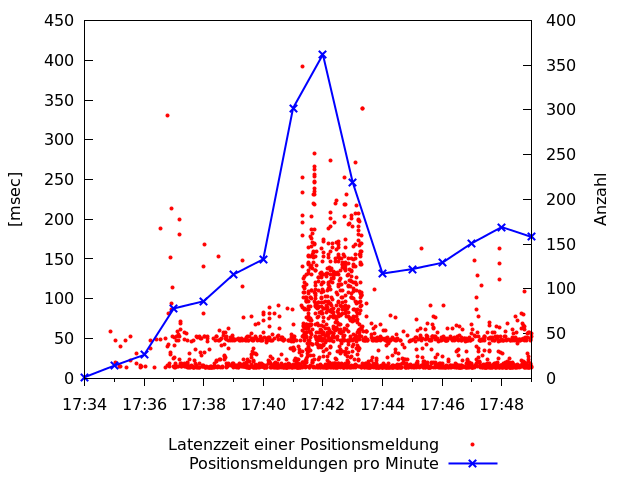
\includegraphics[width=4.5in]{images/latency_timeReceived_socket_io.png}
\end{center}
\caption{socket.io-Websocket-Server: Latenzzeit der Positionsmeldungen und Anzahl empfangener Schiffe}
\end {figure}

\begin {figure}[H]
\begin{center}
  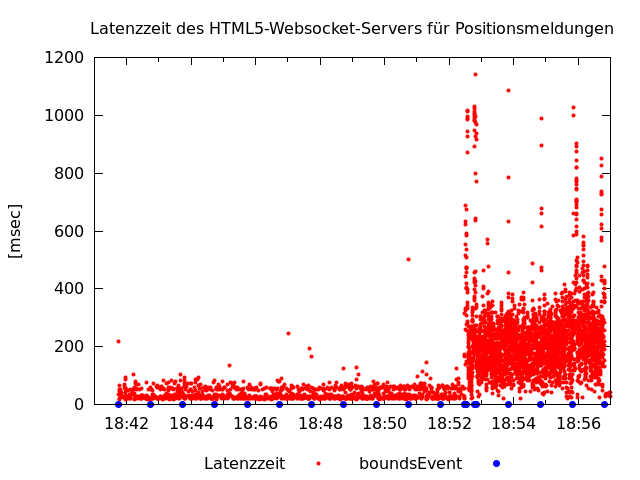
\includegraphics[width=4.5in]{images/latency_timeReceived_HTML5.png}
\end{center}
\caption{HTML5-Websocket-Server: Latenzzeit der Positionsmeldungen und Anzahl empfangener Schiffe}
\end {figure}


\subsection{Performance}
paintToMap

\subsection{Browserunterstützung}
Firefox, Chrome, IE, Safari


\section{Javascript-Client vs. Dart-Client} 
\subsection{Implementierungsaufwand}

\subsubsection{js-Client}
Zeilen Code



\subsection{Latenzzeit}
queryTime

\subsection{Performance}
paintToMap
\newpage

\begin {figure}[H]
\begin{center}
  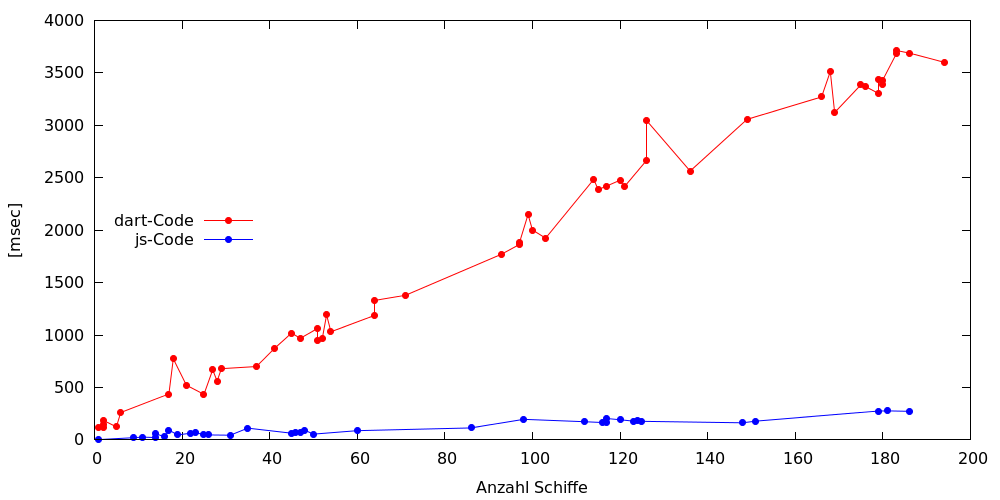
\includegraphics[height=2.3in]{images/Dartium.png}
\end{center}
 \caption{Dauer des Renders in Dartium}
\end {figure}


\begin {figure}[H]
\begin{center}
  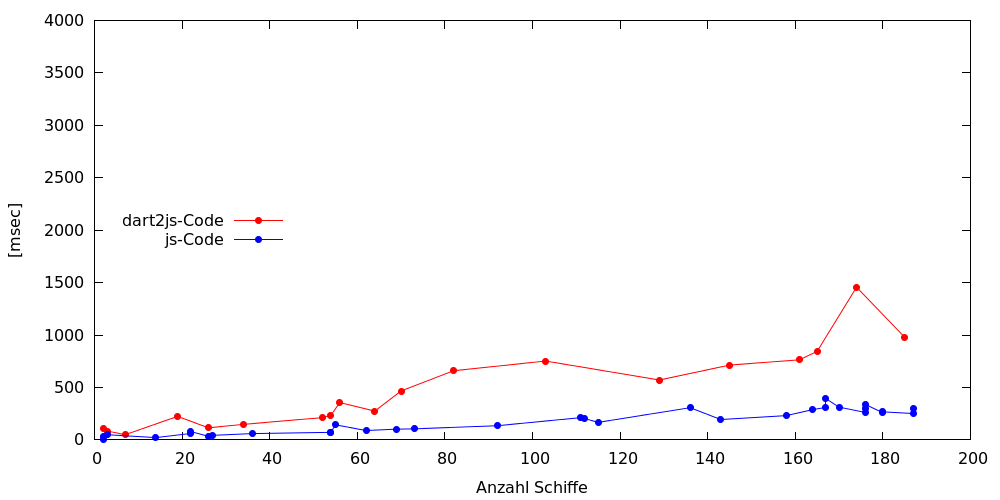
\includegraphics[height=2.3in]{images/Chrome.png}
\end{center}
 \caption{Dauer des Renders in Chrome}
\end {figure}


\begin {figure}[H]
\begin{center}
  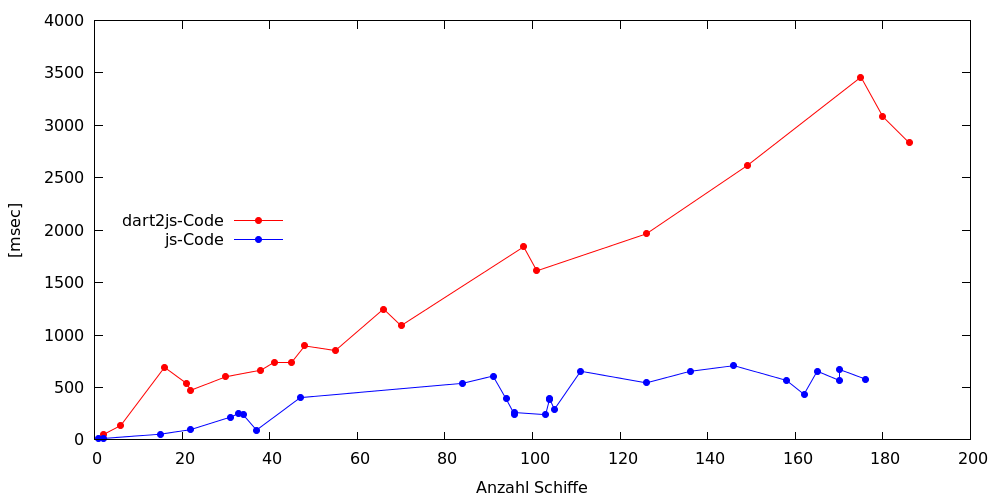
\includegraphics[height=2.3in]{images/Firefox.png}
\end{center}
 \caption{Dauer des Renders in Firefox}
\end {figure}


\subsection{Browserunterstützung}
\subsubsection{Dartium}

\subsubsection{Firefox, Chrome, IE, Safari}

Der dart-Client kompiliert den in Dart geschriebenen Code zu Javascript.

Dabei traten Fehler auf, die unter Dartium (also im originalen Dart-Code) nicht auftraten.
1. Wird innerhalb des Javascript-Scopes eine Methode auf einen javascript-Proxy (hier \_map) aufgerufen und ein proxy wird zurückgegeben, dann ist es nicht möglich auf diesen Proxy, der in diesem Fall vom Typ LatLngBounds sein müsste, eine Methode der Klasse LatLngBounds aufzurufen. => TypeError: t1.get\$\_map(...).getBounds\$0(...).getSouthWest\$0 is not a function

dart-client: web/leaflet\_maps.dart

  List getBounds(){
    var south, west, north, east;
    js.scoped((){
    south= \_map.getBounds().getSouthWest().lng;
        west = \_map.getBounds().getSouthWest().lat;
        north = \_map.getBounds().getNorthEast().lng;
        east = \_map.getBounds().getNorthEast().lat;
 });
return [west, south, east, north];
    
In diesem Fall wird einfach als work-Around eine andere Methode verwendet (getBBoxString), die einen String mit den Bounds zurückgibt. Aus den Teilen dieses Strings werden mit der Methode parse(string) der Klasse double die Werte der Eckpunkte der Bounds generiert.

String getBounds(){
    String bBox;
    js.scoped((){
      bBox = \_map.getBounds().toBBoxString();
    });
    return bBox;
  }

 Weil dadurch der message-Parameter 'bounds' kein number-Array, sondern ein String ist, muss im html5-Server der String einmal zum Float geparst werden.



2. Ein Feld ("IMO") wird auf null und auf > 0 geprüft.


\chapter{Fazit}\label{c.Fazit}

 \section{Ergebnisse }

\section{Ausblick}
-Satellitendaten in die Anwendung einbinden

\bibliographystyle{alphadin_martin}
\bibliography{literatur}
%\begin{thebibliography}{999}
%\bibitem{weranders}
%        "Hans Weranders",
%       "Der Titel ist seine Allegorie seiner selbst",
%        “Bücher über dies und das",
%       "1999",
%        "Februar",
%         "257-286"
%\bibitem {sethladd} Seth Ladd, 
%        {Sorry, at the time of this writing, I'm not aware of a socket.io port for Dart. socket.io is nice because it has a bunch of implementation options for browsers that don't support Web sockets.
%Sounds like a good idea for a hackathon project!},
%       {2012}, {October},{15}
%\bibitem{teixeira}{Pedro Teixeira},
%Professional Node.js,
%{Wrox},
%{2012},
%408 p
%
%\bibitem{demtroeder02}{Wolfgang Demtröder}
%{Experimentalphysik III},
%{Springer Verlag},
%{2002},
%{234-256}
%
%\end{thebibliography}

%---------------------------------------------------------------------------------------------------------------------------------------------
\chapter*{Erklärung}

Hiermit versichere ich, dass ich die vorliegende Arbeit selbstständig verfasst und keine anderen als die angegebenen Quellen und Hilfsmittel benutzt habe, dass alle Stellen der Arbeit, die wörtlich oder sinngemäß aus anderen Quellen übernommen wurden, als solche kenntlich gemacht und dass die Arbeit in gleicher oder ähnlicher Form noch keiner Prüfungsbehörde vorgelegt wurde.

\vspace{3cm}
Ort, Datum \hspace{5cm} Unterschrift\\

\end{document}